\section{OWASP Mobile Security Testing Guide}

	O MSTG é uma guia/manual que descreve como verificar os requisitos listados no MASVS (Mobile Application Security Verification Standard). Descrevendo várias tecnicas gerais e especificas para o sistema operativo de como fazer Tests aos requisitos. Este livro teve vários autores, co-autores, colaboradores grandes e pequenos visto que é um livro open source. Os autores principais são Bernhard Mueller, Jeroen Willemsen e Sven Schleier.
	Seguidamente, serão feitos alguns pontos importantes sobre a natureza das aplicações, hardware onde estas aplicações executam.
	Mobile Apps tem uma superficie de ataque menor, isto é, menos vetores de ataques possíveis do que um sistema completo. Assim prioritiza-se a proteção da informação contida nas Apps e as suas ligações com a rede.
	O cuidado a ter com a informação guardada deve ser grande visto que facilmente os "telemoveis" são robados fisicamente, e também, comunicam com vários sistemas. Isto implica que deve-se usar com precaução as APIs do Sistema Operativo e de IPC( Inter-process Communication) para evitar desvelar informação a outros processos a correr na mesma máquina ou para um sistema de Cloud storage, cache ou similar. Assim, recomenda-se usar APIs recomendada para guardar as Key criptograficas e HSM (Hardware Security Module) se tiverem disponiveis nas últimas versões mesmo que isto implique excluir utilizadores. Em termos de comunicação com o exterior recomenda-se usar protocolos seguros como são o SSL/TLS.
	Ao nivel aplicacional, deve-se ter em contas as vantagens e desvantagens dos diferentes tipos de autentificação sejam estes implementados pelo próprio serviço ou ainda utilizando frameworks de autentificação como OAuth2 (Google, Facebook, Twitter ....). Tendo especial cuidado as APIs especificas que contem os seus próprios problemas e cuidados a ter seja Android ou iOS.
	A comunicação usada pelas aplicações é, na sua maioria, isolada. Assim, estas são mais resistentes a buffer overflow vulnerabilities e XSS (Cross-site Scripting) attacks. Dito isto, ainda se requere que o código siga as melhores práticas para fortalecer a segurança e, por conseguinte, evitar tampering.

\section{Terminologia}

	Nesta seção apresentar-se-á vários conceitos fundamentais para entender o contexto de analise e teste de uma aplicação. O primeiro considera o conhecimento do teste sobre a aplicação a testar, divindo em três conceitos:

\begin{itemize}

\item Black-Box Testing - O tester/test apenas conhece a informação pública sobre a aplicação comportando-se o mais próximo possível de um atacante real.

\item White-Box Testing - Oposto do anterior, o tester conhece a aplicação por completo, isto é, source code, funcionalidades, documentação, diagramas, etc.

\item Gray-Box Testing - Meio-termo. É o mais comum na industria visto que compromete-se no número de testes, etc. Também se compremete no conhecimento disponibilizado ao tester, sendo um compromisso entre o tempo,da completude dos testes.

\end{itemize}

Recomenda-se para um aplicação que não foi testada ainda que se use o White-Box Testing para detetar os problemas de segurança ao nivel do código. Sejam estes ao nivel de segurança ou ao nivel lógico de funcionamento.

A analise destas vulnerabilidades pode ser feita de das seguintes formas:

\begin{itemize}

\item Static Application Security Testing (SAST) - Esta tecnica examina os componentes da aplicação analisando o source code manualmente ou atraves de uma ferramenta que o faça automaticamente. A analise manual pode ser feita de várias maneiras usando metodos como grep para procurar certos comandos especificos que se conheça que possa conter vulnerbilidades. Por exemplo, funções que acedam a uma base de dados. De forma a ajudar o processo pode se usar algumas ferramentas que apontam para possiveis problemas ( IDE + Tools). É útil para quando se quer encontrar problemas lógicos no programa, falhas no design, etc. No entanto este tipo de review é lenta, consome bastante tempo e requer alguem que seja proeficiente tanto na linguagem como nas ferramentas usadas.A analise automatica permite complementar a analise manual. Aponta para problemas e avisos seguindo algumas regras configuradas na ferramenta usada. Os problemas tem que ser revistos por um professional já que é possível haver falsos positivos.

\item Dynamic Application Security Testing (DAST) - Esta tecnica analisa a aplicação enquanto esta está a executar. Principalmente, obtendo informação sobre falhas de segurança não no código mas na interação das varias componentes do mesmo. Por exemplo,encontrar vulnerabilidades no processo de auntentificação e autorização ,como nos padrões dos pedidos e respostas entre ambos os intervenientes,erros de configuração no servidor, etc.


\end{itemize}

O Pentesting consiste em utilizar um leque de ferramentas para testar eludir a segurança implementada na aplicação. É recomendado a utilização do MASVS como base para o teste. A seguir apresenta-se uma lista de passos que devem ser seguidos para os testes procederem com normalidade e efetivamente.

\subsection{Preparation}

	Processo necessário antes de começar os testes. Definir o que se quer testar, que controis de segurança, objetivos dos testes, sensitive data. Acordar com o Cliente o que se pretende fazer requererndo uma autorização escrita para definir os limtes. Os testes a ser realizados, a cobertura dos mesmos e os requisitos que se quer cumprir da lista do MASVS tem que ser discutido com o cliente. Apesar da lista do MASVS Level 1 ser aplicável para as Mobile Apps, o melhor é comunicar com os skateholders. Enquanto ao L2 é necessário rever quais as leis e os regulamentos que podem ser aplicados ao tipo de aplicação que se pretende desenvolver visto que estes requisitos são para aplicações mais criticas.
	Todas as decisões tomadas sobre os requisitos de segurança a serem desenvolvidos/testados tem que ser acordados com o Cliente como justificados num relatorio. Tanto para evitar problemas legais com o mesmo como também para testar todos os requisitos necessários.
	É possivel que existam outras restrições para os testes para a analise dinamica nas instalações do cliente. Por exemplo, não permitirem usar ferramentas de analise da rede por parte do cliente. Uma forma de testar seria usar o Black Box testing para a analise dinamica e requisitar a aplicação em release e em modo debug com algumas funcionalidades desativadas de forma a poder testar os vários requisitos de segurança.
	Outro ponto importante é identificar qual é que é considerado informação sensivel que a aplicação manipula. Para ser possivel testar se existe algum tipo de leak sobre esta informação.Caso não haja um acordo sobre este ponto podem ser considerados os seguintes pontos:

\begin{itemize}

\item Informação de autentificação do utilizador (credenciais, PINs, etc.).

\item Informação que possa ser utilizada para identificar a pessoa, podendo ser utilzada para realizar um roubo de identidade.

\item Informação que apesar de produzida pela aplicação, tem que ser protegida ao abrigo das leis.

\item Informação gerada pela aplicação que é importante para a segurança da aplicação e/ou do próprio sistema.

\end{itemize}

\subsection{Intelligence Gathering}

O processo de recolha de informação deve recolher informação ambiental, isto é, do contexto onde é executada como informação arquitetural. Como informação do primeiro tipo pode ser considerado o seguinte:

\begin{itemize}

\item Os objetivos da aplicação
\item O perfil de risco da aplicação
\item Skateholders e investidores

\end{itemize}

E, como informação arquitetural:

\begin{itemize}

\item Acesso de informação pela aplicação, comunicação com outros processos, gestão das sessões de utilzadores, deteção e reação de jailbroken e rooted phones.

\item Sistema Operativo e versão do sistema operativo em qual a aplicação vai correr. Se é esperado correr em dispositivos que tenhas mobile device Management(MDM) controls e outras vulnerabilidades do sistema operativo.

\item NETWORK: Como usa a rede? Usa protocolos seguros? Usa chaves de tamanho suficiente e algoritmos fortes?

\item Remotes Services: Quais os serviçoes remotos que aplicação usa e se um ataque aos mesmos pode afetar a aplicação.

\end{itemize}


\subsection{Mapeameanto da Aplicação}

Após o security tester ter suficiente informaçao sobre a aplicação como tambem do seu contexto pretende mapear a mesma, ou seja, identificar a estrutura da aplicação, os dados, os pontos de entrada e as funcionalidades. Para tal pode usufruir da documentação existente da aplicação, como , por exemplo, diagramas da arquitetura, especificação funcional, código. De forma a ajudar o security tester é aconselhavel as empresas realizarem Threat Modeling \cite{ref_intro7}. 

Para realmente, realizar o mapeameamento em conjunto com a documentação supra-citada deve-se utilizar tecnicas de SAST, caso seja possivel. E DAST para detetar as os aspetos acima citados como vulnerabilidades seja manualmente ou utilizando ferramentas.

\subsection{Exploitation}

O tester irá testar explorar as vulnerabilidades encontradas nas fases anteriores e analisa-las. Apesar de raramente se chegar a esta fase, permite classificar segundo varias dimensões as vulnerabilidades encontradas. As dimensões normalmente consideradas são as seguintes:

\begin{itemize}

\item Damage potential - o dano resultante de explorar esta vulnerabilidade.
\item Reproducibility - facilidade de reprodução do ataque
\item Exploitability - facilidade para executar o ataque
\item Affected users - O número de utilizadores afetados pelo ataque
\item Discoverability - Facilidade de descoberta da vulnerabilidade

\end{itemize}

\subsection{Reporting}

Todas as vulnerabilidades deve ser devidamente documentadas para que o Cliente perceba qual o impacto da vulnerabilidade encontrada. Existem muitos tipos de templates para fazer report do testing feito. Por exemplo, qual a vulnerabilidade, com que teste foi encontrado, como é que o teste foi executado, a possibilidade da vulnerabilidade ser explorada, o que é comprometido caso seja explorado são só alguns exemplos de dados que podem estar na documentação.

\section{ SDLC - Software Devolpment Life Cycle }

O ciclo completo de SDLC consiste em vários passos que podem ser incorporados num paradigma Waterfall ou no paradigma Agile. Isto é, podem ser adaptados a paradigmas que fazem passo a passo ou incrementais.

\begin{itemize}

\item Risk Assessment - Realizar perfis dos riscos para as diferentes componentes das aplicações. Para tal precisa-se ter em conta o tipo de informação que é armazenada e processado pela aplicação como os regulamentos adjacentes aos mesmos. Ainda deve-se ter em conta se a aplicação pode ser acedida Online ou não. Aqui poderia ser útil as politicas de classificação dos dados tratados.

\item Security Requirements - São determinados em conjuntos dos requisitos funcionais. Pode ser usado o OWASP MASVS para determinar esses requisitos para uma aplicação de telemovel.

\item Secure Design - Threat Modeling - Invés de analisar os assets que tem mais riscos como na fase de risk assessement aqui, enumera-se, identifica-se, classificando conforme a prioridade, e se possível propõem-se possiveis soluções para as Threats encontradas. Podendo ser estabelecidas regras para realizar código seguro, como também as ferramentas e método para realizar os testes de Segurança. Deve-se manter registo e documentação de todos as alterações e novos requisitos determinados em prol da segurança da aplicação. É sugerido que junto com os requisitos junte-se code snippets em vez de guiar o developer por palavras.

\item Secure Implementations - Security Code Reviews, SAST e Secure Unit Testing fazem parte desta fase.

\item Secure Testing -  Seguidamente, aquando da saida do código candidato para release deve-se realizar testes de PenTesting Manual e automaticamente como também DAST.

\item Aceptance/Secure Operations - Passa-se para os skateholders e caso estes aceitem o software, pode transitar para a fase de produção. Passando para equipa de Operações.

\item Decommissioning -  Finalmente, quando acabar a vida útil do software tem que se fazer o Decommissioning, isto é, removido tudo o que se possa em relação a esta aplicação.

\end{itemize}

Note-se que estas fases podem ser adaptadas e/ou omitidas.

\begin{figure}[h!]
\centering
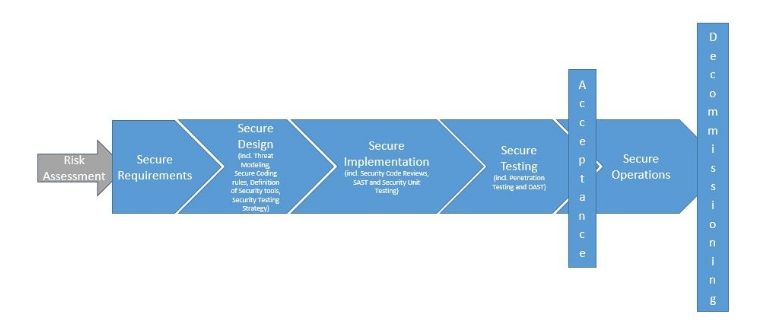
\includegraphics[width=\textwidth]{SDLC.png}
\label{fig:sdlc}
\caption{SDLC}
\end{figure}


\subsection{Definindo uma estrategia de Teste}

	Uma estrategia de teste deve definir quais os tipos de testes a serem realizados como a frequência dos mesmos. Esta estrategia costuma ser definiada apos serem clarificados os riscos e antes da implementação. Outro Input importante é o Threat Modeling executado.
	A estrategia deve ser partilhada pelas diversas equipas envolvidas no projeto visto que a equipa que o define pode nao ser a que a implementa ou pode causar conflitos com algumas delas.
	Para alem de definir quais os testes a serem realizados também define os objetivos com os testes, a descrição dos riscos definidos na fase anterior como qual a importancia dos testes(obrigatorios ou opcionais), quando e como serão executados.
	Para além disso deve-se manter metricas para analisar se a estrategia definida está a ser efetiva. Algumas metricas possiveis são:

\begin{itemize}

	\item Code coverage para os testes unitarios de security controls
	\item Número de bugs de segurança encontrados em cada build apos analise via ferramentas de analise estatica de código.
	
\end{itemize}


\subsection{Security Testing in Waterfall - Agile}

	O modelo Waterfall é sequencial o que causa que os testes, e correção das vulnerabilidades encontradas só irá acontecer depois da aplicação ser desenvolvida e estes erros serão corrigidos com poucas mudanças a arquitetura da aplicação.

	O modelo Agile requer evoluções incrementais do software, ou seja, entregas e desenvolvimento de software. A seguir ir-se-á falar de um cargo importante neste paradigma de software.
	O DevOps é um cargo que implica a colaboração com a equipa de desenvolvimento (DEV) e com a equipa de Operations(OPS). De forma a agilizar o processo de deployment de software, automatizando o processo de build, o processo de testes, de release de softwares e mudanças na infraestrutura(CI/CD). Atualmente, este cargo está a evoluir de tal forma que precisa de colaborar com várias equipas envolvidas no projeto como a equipa de qualidade, de segurança etc... 
	Tendo em vista, o foco principal desta guia focar-se-á no DevSecOps, isto é, adicionar segurança ao processo de DevOps. Os DevSecOps foca-se em minimizar o numero de defeitos da aplicação antes de chegar a produção. Mas também, monitorizar o processo da equipa de Operations para identificar problemas que podem realimentar o processo de desenvolvimento. Dando assim enfase no processo de CI.

	Com o objetivo de conseguir acompanhar a rapidez do processo, necessita-se automatizar o processo principalmente os sub processos essenciais. E abandonar as tarefas que não são produtivas. Focando-se em tres aspetos principais:

\begin{itemize}

\item Infraestructure as Code - A infraestrutra é mantida atraves de scripts, ficheiros de configuração mantidos sobre version control para facilitar partilha e resoluçao de problemas. Por exemplo, ficheiros de configuração para Dockers, maquinas virtuais, etc. Assim, facilita a construção de ambientes de desenvolvimento para as diferentes equipas envolvidas no processo de criação de software.
Alguns recursos Cloud-based providenciam APIs para aceder a items como maquinas virtuais, espeaço de armazenamento e configurações.Ferramentas usadas Puppet, Terraform, Packer, Chef and Ansible.

\item Deployment - A sofistificação do pipeline depende da maturidade da equipa de desenvolvimento. A commit phase normalmelmente involve compiler checks junto com os unit tests associados. Atraves deste sistemas providencia um sistema de feedback para os developers. 
Continuos Integration - Usa o código disponivel para construir o candidato de release. A seguir realiza-se os testes necessários e se forem confirmados pode passar a fase seguinte.
Continuous Delivery -  Após o candidato de release ser avaliado e validado (manual ou automaticamente) o deployment pode continuar.
Continuous Deployment - As releases são passadas para produção sendo disponibilizadas para o utilizador.

\item Security - Os testes de analise estaticos de aplicação podem ser integrado no processo de CI utilizando ferramentas para automatizar o processo. Estabelecendo também Secure Coding Rules. Aquando da release pode ser realizado testes de DAST e, também depois de cada build. Ainda pode-se juntar mais testes manuais no meio das fases. Na fase de Operations deve-se realizar regularmente scans, Pentesting e monitorização ativa de forma de ativar o loop de Feedback.

\end{itemize}

\section{Mobile App Authentication Architectures}


	Os problemas mais prevalentes em termos de segurança são a autentificação e a autorização. Tal pode ser confirmado visto que aparecem no OWASP Top 10 \cite{ref_intro8} em segundo lugar várias vezes.
	Apesar de parte da autentificação e gestão do estado serem mantidos no servidor de backend é importante estudar as implementações mais comuns que podem ser incorporadas em aplicações moveis.
	O tipo de autentificação mais indicada para uma aplicação depende do contexto da mesma, onde vai ser executada, quais os regulamentos que tem de obedecer, etc... Por exemplo, Apps para redes sociais, forums ou similares basta um par username / password com as devidas recomendações para utilização de passwords fortes. Enquanto que uma aplicação com acesso a informação sensivel como é o caso de um banco deve usar 2FA (2-Factor-Authentification) como username/password mais SMS Token. Outra guia possível como já foi referido é usar o MASVS Level 1 para aplcações não criticas e o Level 2 para o outro tipo.
Adicionalmente, pode usar-se a GeoLocation, IP adress e o dispositivo usado para encontrar desvios de comportamento que podem assinalar que a conta do utilizador pode ter sido roubada ou tentativas de fraude.

\subsection{MSTG-ARCH-2 e MSTG-AUTH-1}

Uma das propriedades importantes para testar na autentificação e autorização é se está implementada nos locais corretos. Para tal é preciso ser feito:

\begin{itemize}

\item Identificação de todos os processos de autentificação que aplicação usa.
\item Localização onde estão os endpoints que fornecem uma funcionalidade critica
\item Verificação que existe concordância entre todos os processos de autentificação e os endpoints antes referidos

\end{itemize}

Os servidores devem verificar que o utilizador estã autentificado cada vez que estes requerem um recurso do servidor. Seja atraves das sessões mantidas no servidor ou dos Tokens junto com signatures. Desta forma consegue-se evitar o tampering.

\subsection{MSTG-AUTH-5 e MSTG-AUTH-6}

As passwords usadas pelos utilizadores devem ser fortes para tal deve se implementar uma politica de password. Esta deve obrigar aos utilzadores a escolherem password que cumpre certo número de requisitos de forma a impedir o cracking da password através de métodos manuais ou automáticos.

A OWASP criou uma lista de requisitos para as complexidades das passwords de forma a garantir a segurança das mesmas \cite{ref_intro9}.

Para além disso recomenda-se mostrar os utilzadores a "força" das suas password quando as estão a escolher utilzando bibliotecas como o zxcvbn.

\subsubsection{Login Throttling}

Os atacantes pode tentar descobrir as credenciais de acesso atraves de Brute Force para evitar o mesmo deve ser implementado algumas das seguintes práticas:

\begin{itemize}

\item Bloquear contas temporariamente/permanentemente depois de muitas tentativas falhadas de Login (por exemplo os bancos)

\item Os controls para impedir brute-force deve ser implementados ao nivel do servidor visto que quando implementados ao nivel do cliente podem ser facilmente bypassed.

\item Um conjunto maior de tecnicas para evitar brute force pode ser encontrado no seguinte link da OWASP \cite{ref_intro10}.

\item É so de notar que os sistemas de bloqueio de contas podem causar problemas como DoS para várias contas.

\end{itemize}

Uma forma para testar dinamicamente este sistema de passwords é usar programas como o OWASP ZAP para definir ataques de Brute Force com Dicionario. Para testar contas que se conheça a password utiliza-se uma lista de passwords em que no final está a correta. Caso após algumas tentativas não exista nenhum tipo de bloqueio, temporizador ou captcha pode se concluir que o sistema está suscetivel a ataques por brute-force.


\subsection{MSTG-AUTH-2 e MSTG-AUTH-7}

As Autentificação Session-based pode sofrer ataques de tampering vários por isso também devem ser testados, antes de começar com os cuidados, ir-se-á explicar o fluxo:

1 - App envia um request com as credenciais do utilizador para o servidor

2 - Verifica as credenciais, caso estas sejam válidas uma nova sessão é criada com uma ID gerado aleatoriamente para a sessão.

3 - O servidor envia a resposta que inclui esse ID.

4 - Todas as requests feitas pelo cliente após a auntentificação é adjunto esse Session ID. E o servidor valida e recupera o record associado com essa sessão.

5 - No momento em que o utilzador fizer log out  o record mantido pelo servidor é destruido e o utilizador apaga o Session ID.

Estas sessões devem ser devidamente gerenciadas sendo recomendado o uso de frameworks especializadas no mesmo. Sempre com atenção para os seguintes pontos:

\begin{itemize}

\item Session IDs são gerados aleatoriamente
\item Session IDs são imprevisiveis
\item Session IDs são trocados usando secure connections (HTTPS)
\item Session IDs não são guardados no armazenamento permanente ("Disco")

\end{itemize}

Para complementar o teste a aplicação movel, pode realizar teste ao servidor de back-end seguindo o OWASP Web Testing Guide \cite{ref_intro11} \cite{ref_intro12}

O tempo de vida das sessões devem ser limitado conforme a natureza da aplicação onde vai ser usada. Caso haja acesso ao código pode-se verificar diretamente, caso contrário atraves de um proxy faz-se login numa conta, tenta-se aceder a um recurso tipicamente protegido cada 5 minutos. Quando o servidor devolver um timeout signfica que o timeout está nesse intervalo de 5 minutos. Caso o tempo seja demasiado longo ou inexistente o teste falha. Os tempos de timeout devem pertencer ao intervalo [10, 120] minutos dependendo da aplicação.

\subsection{MSTG-AUTH-4}

O logout incorreto do utilzador é uma falhas mais comuns encontradas. Apesar de ser uma falhas simples pode permitir hijack da conta do utilzador. Isto é possível visto que as sessões não foram devidamente destruidas e os tokens invalidados.

Para testar, caso o código esteja disponivel, deve-se rever a implementação e compara-la com soluções de referência. Caso queira-se fazer uma analise dinamica pode testar fazendo o seguinte:

1 - Log in

2 - Aceder a recurso protegido

3 - Log out

4 - Tentar aceder ao mesmo recurso protegido

A resposta após Log out deve ser um redirecionamento ou um código de erro. Caso contrário significa que o sistema não destroi as sessões / invalida os tokens como pretendido.

\subsection{MSTG-AUTH-9 e MSTG-AUTH-10}

Two-Factor Authentification (2FA) é usada para aplicações que acedem a dados/funções que devem ser mais protegidos. Normalmente, um user/password para o primeiro passo da auntentificação e alguns dos seguintes como segundo:
\begin{itemize}

\item One-time Password via SMS (SMS-OTP)
\item One-time code por chamada telefonica
\item Hardware/Software Token
\item Push notifications em combinação com PKIs

\end{itemize}

Primeiro,e apesar de ser uma prática normal, o uso de SMS-OTP apresentam várias ameaças. Entre elas estão:

\begin{itemize}	

\item A utilização de femtocells para interceptar os SMS

\item Trojans instalados no próprio dispositivo que possa transmitir a mensagem para o dispositivo do atacante, por exemplo.

\item SIM SWAP Attack, isto é, conseguir pedir uma segunda via do cartão SIM pelo atacante.

\end{itemize}

Os problemas anteriores podem ser mitigados ou dificultados para o atacante para tal sugere-se usar alguns dos seguintes mecanismos:

\begin{itemize}

\item Usar o canal dedicado. Usar uma aplicação dedicada para receber este tipo de mensagens que não possam ser acedidas por outras aplicações.

\item Usar autentificadores com maior entropia de forma a fazer os OTPs mais dificeis de advinhar ou descobrir.

\item Utilizar Push Notifications em combinação com PKIs assinando as transações executadas. Exemplo de Funcionamento: A aplicação gera um par chave privada/publica e regista a publica no servidor de back-end. A chave privada é guardada na KeyStore/KeyChain. Finalmente para processar a transação, o servidor envia a informação da transação para o utilizador, este confirma-a, desbloqueia com uma password ou fingerprint o KeyStore/KeyChain de forma a obter a chave privada. De seguida, assina a transação com a chave privada, permitindo o servidor verificar com a chave pública.

\end{itemize}

	Um dos testes possíveis a segurança deste mecanismo seria testar os 2FA e interceptar as requests. Realizar replays attacks a partir das requests intercetadas. Testando se é possivel aceder a recursos defendidos por esta autentificação. Caso o sistema responda quer dizer que o sistema não é seguro.
	O OTP requere que se bloquei após varias tentativas falhadas. Uma forma de testar é antes de enviar o código correto enviar 10-15 tentativas erradas. Caso o sistema não bloqueie antes da correta é considerado inseguro.


\subsection{ MSTG-AUTH-3 }

A autentificação por tokens resulta de enviar tokens assinados/verificados pelo servidor com cada HTTP request. Estes tokens são divididos em três partes: o header, o payload e a assinatura.

O header é composto pelo nome do algoritmo usado e o tipo do token. O payload contem informação sobre o utilizador e metadata. O último valor é a assinatura que é calculada da forma Alg(header,payload,secret\_value). O segredo é partilhado entre o servidor de auntentificação e o servidor de backend ficando escondido do utilizador.

Numa perspetiva estatica de analise convêm verificar as seguintes propriedades como outros que não estão aqui listadas:

\begin{itemize}

\item Verificar que o HMAC é verificado em todos os requests que chegam.
\item Verificar que a chave privada como a chave secreta HMAC estão disponiveis só para o "emissor" da assinatura e o "verificador".
\item Verificar que os ataques por repetição são tratados pela utilização de JWT ID.
\item Verificar que os tokens são guardados seguramento no dispositivo como, por exemplo, KeyChain/KeyStore.

\end{itemize}

É importante que os Tokens tenham uma expiration date ou ainda implementar-se um esquema de acess tokens e refresh tokens.

Numa analise dinamica pode-se tentar fazer:
\begin{itemize}

\item Brute-Force da chave secreta offline utilizando ferramentas como John The Ripper.

\item Decodificar a base64 do JWT e verificar que tipo de informação é transmitida e se esta encriptada. É suposto que se existir informação sensivel esteja encriptada. 

\item Verificar se mudanças no header não resultam em Tokens validos com assinaturas forjadas.

\end{itemize}

\section{Cryptography for Mobile Apps}

\subsection{MSTG-CRYPTO-4}

Os algoritmos usados nas várias aplicações devem ser revistos com regularidade. Isto para que os algoritmos que estão a ser utilzados sejam alterados, o tamanho das chaves usadas atualizadas segundo as recomendações, as chaves são usadas cada uma para o seu propósito, isto é, a chave usada para HMAC deve ser diferente da chave usada para encriptação.

\subsection{MSTG-CRYPTO-1, MSTG-CRYPTO-2 e MSTG-CRYPTO-3}

A seguir apresenta-se vários conselhos que servem tanto para aplicações moveis como quase para qualquer tipo de aplicação que utilize mecanismos de criptografia.
\begin{itemize}

\item Assegurar-se que as chaves usadas nas aplicações não são guardados nos mesmos sitios que a informação que é encriptada/assinada/etc.

\item Recomenda-se não usar chaves estaticas compiladas diretamente no código visto que com ajuda de um disssambler consegues descobrir facilmente. A ofuscação do código também pode ser desfeita usando dynamic instrumentation.

\item A password do certificado deve ser guardada no Keychain caso sejam utilzados (Two-way SSL).

\item Uma forma de usar a password é usa-la como chave. Recomenda-se passar por uma KDF antes com pelo menos 10,000 iterações para gerar a chave a ser usada.

\item Deve-se evitar sempre o uso de funções criptograficas "caseiras" e optar por API Standard das plataformas escolhidas. As implementações não standard deve ser cuidadosamente analisadas, tendo em conta que os calculos intermedio de chaves e o estado interno da cifra tem que desaparecer da memória o mais rápido possivel.

\item Caso escolha-se o AES como encriptação deve-se escolher o modo de operação seguro, ou seja, evitar ECB, por exemplo. Seguir as recomendações sobre os IV/Nonces usados e ter em conta os ataques possíveis aos mesmos. E acompanhar com mecanismos de integridade, etc.

\item Escolher um bom mecanismo de Padding. Evitando o uso de PKCS\#5/7 e usar outros como o OAEP.  

\item Aquando do transporte de chaves entre dispositvos deve-se usar os mecanismos corretos. Por exemplo, criptografia assimetrica ou Key encapsulation mechanisms.

\end{itemize}

\section{Testing Code Quality}




O código tem que ser testado a sua qualidade visto que a mistura de frameworks e linguanges num projeto pode levar a algumas falhas como SQL Injection, buffer overflows e XSS.

\subsection{MSTG-ARCH-2 e MSTG-PLATFORM-2}

Uma falha de injeção de código refere-se quando algo que o utilizador escreve, seja isto diretamente do utilizador ou um processo é passado a um comando ou a uma query de backend resultando em comportamento não esperado.

Um caso tipico seria os casos de SQL Injection ou os XML Injection. Uma forma de testar passa pelo seguinte tendo em conta os canais mais perigos como a UI, IPC calls, QR Codes:

\begin{itemize}

\item Identificar entradas de untrusted Input e ver se é possivel executar funções que podem conter informação importante no alcance desse Input.

\item Identificar API e biblitecas que tenham comportamento perigoso caso o Input não seja devidamente visto ou "arranjado".

\item Deve-se usar Prepared Statments para separar a informação definida pelo o utilizador e o código.


\end{itemize}

\subsection{MSTG-CODE-8}

Os erros associados a corrupção de memória ate são comuns e pode ocorrer de várias formas. Os atacantes podem aproveitar-se disso para controlar o fluxo do programa e saltar certas condições de segurança ate injetar código pretendido. A seguir apresenta-se alguns problemas que causam este tipo de Bugs:

\begin{itemize}

\item Buffer Overflows - Descreve um erro que consistem em escrever depois de acabar o range de memória de certo objeto. Podendo apagar certas variaveis e apontadores para funções manipulando o fluxo como pretendido. Hoje em dia são mais raros porque já existe mais consciência sobre este tipo de problemas como também são faceis de detetar.

\item Use-after-free - Refere-se a utilização de pointers que apontam para memória já libertada. Podendo mais tarde este apontador referenciar outros objetos válidos.

\item Integer Overflows - Dependendo o que o inteiro represente pode ser útil para atacar o sistema provocar um Overflow ou Underflow.

\item Format String - Deixar o utilizador aceder as Formats Strings sem nenhum tipo de controlo pode causar em comportamento malicioso por parte do utilizador inserindo tokens para aceder a memória.

\end{itemize}

O teste para encontrar este tipo de vulnerabilidades pode ser intricado, mesmo usando ferramentas automáticas a não ser casos simples (RATS). Por isso, a forma mais eficaz de encontrar este tipo de vulnerabilidades é usar "Fuzzers" scripts que constroem estruturas semi bem formadas (Desde o Inicio ou mutando por uma estrutura antes válida). Envia-nas para a aplicação, ficando a escuta caso haja algum erro na aplicação. Cobrindo uma grande percentagem dos vários execution paths.

\section{Tampering and Reverse Engineering}

Reverse Engineering refere-se ao processo de analisar a aplicação compilada para extrair informação sobre o código fonte.Tampering refere-se ao processo de alterar a aplicação ou o ambiente de forma a afetar o comportamento da mesma. Por exemplo, alterar para poder correr certos tipos de testes.Ao misturar os dois pode-se moldar uma aplicação para realizar/permitir operações em prol do nosso interesse.Algumas vantagens do Reverse Engineering:
\begin{itemize}

\item Black-Box Testing - Apps modernas incluem mecanismo que previnem de interceptar or manipular trafégo com proxys ou Root Detection. Deve ser possivel desactivar essas defesas para realizar os testes.

\item De forma a facilitar a analise statica da aplicação. Ate pode-se encontrar credenciais hardcoded.

\item Para verificar a resistencia da própria aplicação ao reverse engineering. Para o tal o tester pode executar um resilience assessement como parte do teste geral de segurança.

\end{itemize}

\subsection{ Basic Tampering Techniques }

Binary Patching: alterar binarios já compilados, ficheiros por completo. Por exemplo, decompilar o código, editar e fazer re-assemble. Hoje em dia o processo é mais complicado porque o código vem assinado.Code Injection: modificar processos em execução atraves de ferramentas que permitem descobrir as library que estão loaded, funcões hooked, injetar código,etc . 

Existem várias ferramentas para realizar esta tarefa. Uma das mais versáteis e completas é a Frida.

A ferramenta, rapidamente, injeta código escrevendo diretamente na memória do processo. Atraves do ptrace faz hijack to processo, localizando o chunk de memoria. Seguidamente, carrega a library do agente da Frida e estabelece comunicação com a ferramenta. A thread volta ao fluxo normal apos de retornar ao estado original.

Para alem do funcionamento normal ainda existem mais modos disponiveis para execução desta ferramentas, como widgets e tools adicionais para acrescentar funcionalidades. Ou, ainda, outras ferramentas desenvolvidas a partir desta.

Disassemblers e Decompilers permitem reconstruir o código para um formato mais ao menos legivel para o tester. Assim, ganhando conhecimento de como o programa funciona e o fluxo que este tem.
Podendo juntar-se ao processo Debugging e Tracing para analisar o programa em execução, o primeiro para analisar o estado interno, definir breakpoints enquanto que o segundo permite recuperar informação sobre quais a execução da aplicação como as call a API.

\section{Testing User Interaction}

\subsection{MSTG-STORAGE-12}

Os utilizadores devem ser informados dos seus direitos, mais concretamente, do GDPR na Europa como os direitos associados ao mesmo. Como por exemplo, o direito a ser esquecido, o direito a correção da sua própria informação e o direito de aceder aos dados guardados pela aplicação sobre o utilzador.

Os utilizadores tambem deve ser informados dos perigos e melhores práticas de segurança sempre que pertinente.


